\pagestyle{empty}

\section*{The Setting}
We work in a compact, riemanian, orientable, smooth Manifold $(M,g)$ of dimension $m$ together with a Morse-Smale funktion 
\begin{align}
    f: M\to \R
\end{align}
We assume that $q$ is a critical point of index $k+1$ and $p$ is a critical point of index $k$. we define $f(q)=b$ and $f(p)=a$ and assume that there is no kritical point in $f^{-1}(a,b)\subseteq M$. We define the sub and superlevelsets 
\begin{align}
    M^t:=\{ x\in M | f(x)\leq t \} \quad \text{and}\quad M_t:=\{ x\in M | f(x)\geq t \} \, ,
\end{align} and the constants 
\begin{align}
    c \in (a,b) \quad , \quad \epsilon >0 \text{ small } \quad,\quad T>0 \text{ big .}
\end{align} With this we define the sets: 
\begin{align}
	N_q  & \coloneq    \{ x\in M_c |f(\phi_{-T}(x))  \leq b+ \epsilon  \}   \, ,  \\
	L_q  & \coloneq    \{ x\in N_q |f(x)             =    c            \}    \, , \\
	N_p  & \coloneq    \{ x\in M^c |f(\phi_T(x))     \geq a-\epsilon   \}    \, , \\
	L_p  & \coloneq    \{ x\in N_p |f( \phi_T(x))    =    a-\epsilon   \} \, ,
\end{align} and finally: 
\begin{align}
	C  & \coloneq  N_p \cup N_q  \, ,                     \\
	B  & \coloneq  N_p \cup L_q   \, ,                   \\
	A  & \coloneq  L_p \cup \mathring{(L_q-N_p)} \, .
\end{align}
\begin{lemma}
    We claim that 
    \begin{enumerate}
	\item $(N_q,L_q)$ is a regular index pair for $q$\, . \label{lem: enum: 1}
	\item $(C,B)$ is an index pair for $q$\, .\label{lem: enum: 2}
	\item $(N_p,L_p)$ is a regular index pair for $p$\, .\label{lem: enum: 3}
	\item $(B,A)$ is an index pair for $p$\, .\label{lem: enum: 4}
    \item $N_p$ is a tubular neighbourhood of $W(\to p)\cap M^c$\, .\label{lem: enum: 5}
\end{enumerate}
\end{lemma}
\begin{lemma}
	Let $\psi:U\to V$ be a chart. Then the gradient has the local form:
	\begin{align*}
		\grad(f)\circ \psi{-1} =\sum_{i,j}g^{ij} \frac{\partial f \circ \psi^{-1}}{\partial x^i} \frac{\partial }{\partial x^j}
	\end{align*}
	Here, $g^{ij}$ denotes the smooth functions given by the coordinates of the function $x\mapsto (g_{ij}(x))$ that defines the coordinate representation of the gradient in $x$. 
\end{lemma}
\begin{proof} Assume that $v,w\in \Gamma( TM)$ such that $v=\sum_i v^i\frac{\partial	}{\partial x^i}$ and $w=\sum_i w^i\frac{\partial	}{\partial x^i}$. Then  $g(v,w)=\sum_{i,j} g_{ij} v^i w^i$.
Suppose that $\grad(f)=\sum_j G^j \frac{\partial}{\partial x^i}$ and $q$ is the coordinate map $T\R\to \R$ in each tangend space. Then by definition of the gradient we have:
\begin{align*}
\frac{\partial }{\partial x^j}(f)=	q \circ \diff f (\frac{\partial }{\partial x^j})=q\circ \frac{\partial f}{\partial x^j}= g(\grad(f),\frac{\partial }{\partial x^j})= \sum_{ij}g_{ij} G^j
\end{align*}Hence, 
\end{proof}

\begin{definition}[Jacobian of the Gradient]
	The gradient is a section into the tangent bundle, $\grad(f):M\to TM$.
	Let $\psi: M\supseteq U\to V \subseteq \mathbb{R}^m$ be a chart. The coordinate map $q_{\psi}$ on $TU$ assigns to a vector $v \in T_pM$ (where $p \in U$ with $\psi(p) = x$) its components with respect to the basis $\left(\frac{\partial}{\partial x^i}\big|_p\right)$, i.e., $q_{\psi}(v) = (v^1, \ldots, v^m)$ if $v = \sum_{i=1}^m v^i \frac{\partial}{\partial x^i}\big|_p$.
	We define the Jacobian of the gradient with respect to the chart $\psi$ as the Jacobian matrix of the coordinate representation of the gradient in this chart:
	\[
	J(\grad(f))_\psi(x) \coloneq J\left(q_{\psi}\circ \grad(f)\circ \psi^{-1}\right)(x) = \left(\frac{\partial (q_{\psi}\circ \grad(f)\circ \psi^{-1})_i}{\partial x_j}(x)\right)_{ij}
	\]
\end{definition}
\begin{lemma}
	Let $g$ be a metric and $\phi_t(x)$ be the flow associated to $-\grad(f)$ meaning
	\begin{align*}
		\frac{\diff}{\diff t}\big|_{t_0}\phi_t(x)=-\grad(f)(\phi_{t_0}(x))
	\end{align*} Let furthermore, $\psi:U\to V$ be a chart. If $t_0$ is small enough and $x\in U$ such that $\phi_t(x)\in U$, then 
	\begin{align*}
		\frac{\partial}{\partial t} \psi \circ \phi_{t_0}(\psi^{-1})(x)=	
	\end{align*}
\end{lemma}

\begin{lemma}
	Let $t\in \mathbb{R}$ be small enough and $\phi_t: M\to M$ be the flow map corresponding to the negative gradient. Assume that $U$ is the domain of a chart $\psi$ and $p\in U$ such that $\phi_t(p)\in U$. Then the linear map $\mathrm{d} \phi_t \big|_p: T_pM\to T_{\phi_t(p)}M$ has a local representation in the coordinates induced by $\psi$ given by:
	\[
\frac{\partial}{\partial x} \psi \circ \phi_t(\psi^{-1}(x))=\exp\left(- q_{\psi} \circ \grad(f)\psi^{-1} \cdot t \right) \, .
	\]
\end{lemma}
\begin{proof}
For this we consider the function $ (t,x)\mapsto \psi \circ  \phi_t(\psi^{-1}(x)):\R \times U \to U$ For fixed $x$ we can calculate
\begin{align*}
	q_{\psi}\frac{\diff}{\diff t} \phi_t(\psi^{-1}(x))=-q_{\psi} \circ \grad(f)(\phi_t(\psi^{-1}(x)))
\end{align*} and by changing the order of integration we have:
\begin{align*}
	\frac{\partial}{\partial t}   \frac{\partial}{\partial x} \psi \circ \phi_t(\psi^{-1}(x))
	&= \frac{\partial}{\partial x}   \frac{\partial}{\partial t} \psi \circ \phi_t(\psi^{-1}(x))\\
	&= \frac{\partial}{\partial x} q_\psi \frac{\diff }{\diff t}  \phi_t(\psi^{-1}(x))  \\
	&= -\frac{\partial}{\partial x} q_{\psi} \circ \grad(f)(\phi_t(\psi^{-1}(x)))	\\
	&= -\frac{\partial}{\partial x} q_{\psi} \circ \grad(f)\left(\psi^{-1}\circ \psi\circ \phi_t(\psi^{-1}(x))\right)\\
	&=-\frac{\partial}{\partial x} \left( q_{\psi} \circ \grad(f)\circ \psi^{-1} \right)\frac{\partial }{\partial x}  \left(\psi\circ \phi_t(\psi^{-1}(x))\right)
\end{align*}
Hence by the theory of linear differential equation with $\frac{\partial}{\partial x} \psi \circ \phi_0(\psi^{-1}(x))=1_m$ we have:
\begin{align*}
	\frac{\partial}{\partial x} \psi \circ \phi_t(\psi^{-1}(x))=\exp\left(- q_{\psi} \circ \grad(f)\circ \psi^{-1}\cdot t \right) \, .
\end{align*}
\begin{comment}
\begin{align*}
		q_{\psi}	\frac{\partial}{\partial x} \phi_t(\psi^{-1}(x))=\exp\left( q_{\psi} \circ \grad(f)\psi^{-1} \right) \, .
	\end{align*}
\end{comment}

\end{proof}













\begin{lemma}
	Let $\psi$ be a coordinate system arround a critical point $p$. I.e. $\psi: p\in U\to V$ with $\psi(p)=0$ and let $\left( \frac{\partial}{\partial x_1}\big|_x,\dots ,\frac{\partial}{\partial x_m}\big|_x\right)$ be the induced basis of $T_xM$ Then the jacobean of the gradient 
	\begin{equation}
			J(\grad(f))_\psi(0)= \sum_{k}g^{ki}(0)\frac{\partial ^2 f\circ \psi^{-1} }{\partial x_j \partial x_k}
	\end{equation} where $(g^{ki}(x))$ denotes the matrix corresponding to the gradient in $T_xM$ with respect to the basis $\left( \frac{\partial}{\partial x_1}\big|_x,\dots ,\frac{\partial}{\partial x_m}\big|_x\right)$.
\end{lemma}
\begin{proof}
	Let $q_{\psi}$ denote the koordinate funktion $TU\to R^m$ induced from the basis $\left( \frac{\partial}{\partial x_1}\big|_x,\dots ,\frac{\partial}{\partial x_m}\big|_x\right)$. then the gradient in $\psi$ reads:
	\begin{align*}
		q_{\psi}\circ \grad(f)=\left(\sum_kg^{k1  }\frac{\partial f\circ	}{\partial x_k},\dots, \sum_kg^{k m }\frac{\partial f\circ	}{\partial x_k}\right)
	\end{align*}
	Hence, we can differentiate: 
	\begin{align*}
		\frac{\partial}{\partial x}  Q\circ \grad(f)\circ \psi^{-1}
		&= \left(\frac{\partial}{\partial x_j} \sum_k g^{ki}\frac{\partial f \circ \psi^{-1}}{\partial x_k}\right)_{ij} \\
		&= \left(\sum_k \left[ 
		\frac{\partial g^{ki}}{\partial x_j}\frac{\partial f \circ \psi^{-1}}{\partial x_k} +  g^{ki}\frac{\partial^2 f \circ \psi}{\partial x_j ~\partial x_k}
		\right]\right)_{ij} \, .
	\end{align*}
	and now in $p=\psi^{-1}(0)$ we have
	\begin{align*}
		\frac{\partial}{\partial x}  Q\circ \grad(f)\circ \psi^{-1} \Big|_{0}=\left(\sum_k \left[ 
		g^{ki}(0)\frac{\partial^2 f \circ \psi^{-1}}{\partial x_j ~\partial x_k}
		\right]\right)_{ij} \, .
	\end{align*}
\end{proof}








\begin{theorem}[Sylvesters Law of Inertia]
Let $A\in \Mat(n,\R)$ be symmetric and let $T,T'\in \GL(n,\R)$ and $k,k',l,l'\in \N$ such that \\
\begin{align*}
T^t\circ A\circ T=	\begin{pmatrix}
		1_k& 0 &0\\
		0& -1_l&0\\
		0&0&0_{n-k-l}
	\end{pmatrix}\text{ and } 
	T'^T\circ A \circ T'=
	\begin{pmatrix}
		1_{k'}& 0 &0\\
		0& -1_{l'}&0\\
		0&0&0_{n-k'-l'}
	\end{pmatrix}
\end{align*}
then $k=k'$, $l=l'$ and $\rank(A)=k+l.$
\end{theorem}
\begin{proof}
	Since $T,T'$ are invertible we have that
	\begin{align}
		k+l=\rank(T^t\circ A\circ T)=\rank(A)=\rank(T'^T\circ A\circ T')=k'+l' \, .
	\end{align} Hence it suffices to show that $k=k'$. Which we will do by proofing the claim:
	\begin{equation*}
		k=\max \left\{ \dim(U)|U\subseteq \R^n \text{subspace such that } x^tAx>0 ~\forall x\in U\setminus \{0\}  \right\}
	\end{equation*}
	So we start by showing \glqq $\leq $\grqq:
	Denote the first $k$ colomus of $T$ with $x_1,...,x_k$. They form a basis of $\R^n$ and with $ 0 \neq x=\sum_{i=1}^k\lambda ix^i$ we have that by bilinearity
	\begin{equation}
		x^TAx=\sum_{i=1}^{k}\lambda_i x_i^T A x=\sum_{i,j=1}^{k}\lambda_i \lambda_j x_i^T A x_j=\sum_{i=1}^{k}(\lambda_i)^2\geq 0 \,. 
	\end{equation} This conculdes the first inequality. 
	
	Now let $U$ be any $k-$dimensional subspace such that for all non zero $x\in U$ $x^TAx>0$. By a calculation analog to the one above we have that for any $x\in W:= \gen (x_{k+1},\dots x_n)$ the number $x^tAx$ is less or equal to zero. Hence, $W\cap U= \{0\}$ and with this we conclude:
	\begin{equation}
		\dim(U)=\dim(U+W)-\dim(W)+\dim(U\cap W)\leq (k+(n-k))-(n-k)+0=k\, .
	\end{equation} This is the last inequality proving the statement.
	\end{proof}
\begin{lemma} \label{lem: linear chart change and tangend basis change}
	Assume that $\psi:U\to V$ is a chart and $L:R^m\to R^m$ a linear function.
	Then the diagramm \begin{center}
		% https://tikzcd.yichuanshen.de/#N4Igdg9gJgpgziAXAbVABwnAlgFyxMJZABgBpiBdUkANwEMAbAVxiRABUB9NAWRAF9S6TLnyEUARnJVajFmwA6CgEoA9ALYChIDNjwEiUiTPrNWiEErWb+MmFADm8IqABmAJwibEZEDghIUrJmbACOnMBKaNj8AD7cWm6e3r7+SABM1KbyFuHAADJKAMZY7kUABFEx8Wgg1Ax0AEYwDAAKIvriIO5YDgAWOIkgHl6B1GmImcE5IPkCFPxAA
		\begin{tikzcd}
			T_pM \arrow[r, "q_{\psi}|_p"] \arrow[rd, "q_{L\circ \psi}|_p"'] & \R^m \arrow[d, "L"] \\
			& \R^m               
		\end{tikzcd}
	\end{center}  
	commutes for all $p\in U$.
\end{lemma}
\begin{proof}
	We show this by showing the inverse: For any $v\in \R^m$ we have the two $(q_{\psi} \big|_p)^{-1} \circ  L^{-1}(v)$ and $(q_{\psi \circ L}\big|p)^{-1}$ and claim that they are the same. Assume that $L^{-1}=(\lambda_{ij})_{ij}$, $\psi(p)=x_0$, $L(x_0)=\tilde{x_0}$, $(v^1,\dots v^m)=v\in \R^m$ and denote the basis of $T_pM$ coming from the chart $\psi$ by $\left(\frac{\partial}{\partial x^i}\big|_p \right)_i$ and the one coming from $L^{-1}\circ \psi$ by $\left(\frac{\partial}{\partial \tilde{x}^i}\big|_p \right)_i$. We now calculate for $f_p\in \mathcal{E}_pM$:
	\begin{align*}
		\left[(q_{\psi \circ L}\big|_p)^{-1}(v)\right](f_p)
		&= \sum_i v^i \frac{\partial}{\partial \tilde{x}^i}\big|_p (f_p)  \\
		&=\sum_i v^i \frac{\partial}{\partial x^i}\big|_{\tilde{x}_0} (f\circ \psi^{-1}\circ L^{-1}) \\
		&=\sum_{i}v^i \sum_{j} \frac{\partial f\circ \psi^{-1}	}{\partial x^j}\big|_{x_0} \cdot \frac{\partial L^{-1}_j}{\partial x^i}\big|_{\tilde{x_0}}\\
		&= \sum_{i,j}v^i \frac{\partial }{\partial x^j}\big|_{p}(f_p) \cdot \lambda_{ji}\\
		&= \sum_{i,j}v^i q_{\psi}\big|_p^{-1}(e_j)(f_p) \cdot \lambda_{ji}\\
		&= \left[q_{\psi}\big|_p^{-1}(\sum_{i,j} v^i \lambda_{ji} e^j)\right](f_p)\\
		&= \left[q_{\psi}\big|_p^{-1}(L^{-1}(v))\right](f_p)
	\end{align*}
	This concludes the proof.
\end{proof}

\begin{theorem}[Simultaneous Diagonalisation of Quadratic Forms]
	Let $p$ be a critical point of a Morse function $f$ on a manifold $M$ and let $g(p)$ be the Riemannian metric on $T_pM$. Then there exists a Morse chart $\psi$ arround $p$ such that the representation of $g(p)$ in the basis induced by the Morse chart is given by a a diagonal matrix $diag(\mu_1,\dots \mu_m)$ with $\mu_i>0$ for all $i$ .
\end{theorem}
\begin{proof}
	The quadratic form of $f \circ \psi^{-1} - f(p)$ in the coordinates of any Morse chart $\psi$ is $q_H(v) = v^T H v$. The quadratic form induced by the Riemannian metric $g(p)$ is $q_G(v) = v^T G v$, where $v \in \mathbb{R}^m$ are the coordinate vectors with respect to the Morse chart. 
	To be precice this means for $v,w\in \R^m$:
	\begin{align*}
		g\circ ( q_{\psi}\big|_p\oplus q_{\psi}\big|_p ) (v,w)=v^TG w \text{ and } f\circ \psi^{-1} (v)=f(p)+v^T H v \, .
	\end{align*} We now aim to manipulate $\psi$ such that $G$ becomes diagonal:
	Since $g(p)$ is positive definite, $G$ is also positive definite, and $H$ is symmetric.
	
	Consider the generalized eigenvalue problem $Hv = \lambda G v$. Since $H$ and $G$ are real symmetric matrices and $G$ is positive definite, this problem has $m$ real eigenvalues $\lambda_1, \dots, \lambda_m$ and corresponding eigenvectors $v_1, \dots, v_m$, which can be chosen to be orthogonal with respect to the bilinear form defined by $G$, such that $v_i^T G v_j = \delta_{ij}$, since if $v_i$ and $v_j$ are different eigenvectors with respect to different eigenvalues, we can calculate:
	 \begin{align*}
	 	v_j^THv_i=(Hv_j)^Tv_i=\lambda _j(Gv_j)^Tv_i=\lambda _j v_j^T G(v_i)  \quad \text{and}\quad 	v_j^THv_i= v_j^T \lambda_i G(v_i)=\lambda_i v_j^TG(v_i) \, .
	 \end{align*} Hence we have the equality
	 \begin{align*}
	 	\lambda _j(Gv_j)^Tv_i=\lambda_i v_j^TG(v_i) \Leftrightarrow \underbrace{(\lambda_j-\lambda_i)}_{\neq 0}v_j^T G(v_i)=0
	 \end{align*} Hence all eigenspaces are orthogonal and we can use Gram Schmitt to make the bases of the eigenspaces orthogonal and by rescaling orthonormal.
	
	Let $L = [v_1 | \dots | v_m]$ be the matrix whose columns are these $G$-orthonormal eigenvectors. The linear change of coordinates 
	 $y = Lz$ leads to new coordinates $z$. In these new coordinates, the quadratic forms transform as follows:
	\begin{align*}
		q_G(y) &= y^T G y = (Lz)^T G (Lz) = z^T L^T G L z = z^T I z = \sum_{i=1}^m z_i^2 \\
		q_H(y) &= y^T H y = (Lz)^T H (Lz) = z^T L^T H L z
	\end{align*}
	Since $H v_i = \lambda_i G v_i$, we have $L^T H L = \text{diag}(\lambda_1, \dots, \lambda_m)$. The eigenvalues $\lambda_i$ are real and have the same signature as the eigenvalues of $H$ ($l$ negative, $m-l$ positive).This is true to sysvesters law of inertia.  By a further scaling of the $v_i$ and a reordering the matrix $L^T H L$ can be brought into the form $\text{diag}(-1, \dots, -1, 1, \dots, 1)$. (by doing this however, the matrix $L^TGL$ becomes $L^TGL=\diag(\mu_1,\dots \mu_m)$ with $\mu_j>0~\forall j$). If $\psi$ is the Morse chart we started with, then $L^{-1} \circ \psi$ is the new Morse chart: 
	\begin{equation*}
		f\circ (\psi^{-1}\circ L)(y)=f\circ \psi^{-1}(L(y))=q_H(L(y)=\sum_{i=1}^l-y_i^2+\sum_{i=l+1}^my_i^1
	\end{equation*}
	Furthermore, we want to inspect the metric $g\big|_p:T_pM^2\to \R$ with respect to the chart $ L^{-1}\circ \psi $-induced basis $\left( \frac{\partial}{\partial x^1}\big|_p,\dots ,\frac{\partial}{\partial x^m}\big|_p\right)$. By the lemma \ref{lem: linear chart change and tangend basis change}
	\begin{align*}
		g(q_{L^{-1}\circ \psi}\big|_p^{-1},q_{L^{-1}\circ \psi}\big|_p^{-1})(v,w)=	g(q_{\psi}\big|_p^{-1},q_{\psi }\big|_p^{-1})(Lv,Lw)=(Lv)^T G LW=v^T L^TGLw	
		\end{align*}
\end{proof}



\begin{proof}
    The statements \ref{lem: enum: 1}-\ref{lem: enum: 4} are easy to proof by the definitions. The regularity can be derived from a general fact for pairs $(X,Y)$ in metric spaces: If $Y$ is closed in $X$ and there is a neighbourhood of $Y$ that is open in $X$ such that $Y$ is a strong deformation retract of $U$. So the only thing left to show is, that $N_p$ is a tubular neighbourhood. in \cite{MorseTheorySalmbon} in the proof of lemma 3.2 Salamon claims this to be true without a proof (page 119 in the attached source). Similar, in \cite{banyaga2004lectures} Banyaga claims this (also without any argument).
  I find this difficult to proof, since we cannot use the flow for the map from the normal bundle, as points leave $N_p$ along the flow: The Set $N_p$ is sketched in the figure below. 
    \begin{center}
        

\tikzset{every picture/.style={line width=0.75pt}} %set default line width to 0.75pt        
\resizebox{\linewidth}{!}{%



\tikzset{every picture/.style={line width=0.75pt}} %set default line width to 0.75pt      

\tikzset{every picture/.style={line width=0.75pt}} %set default line width to 0.75pt        

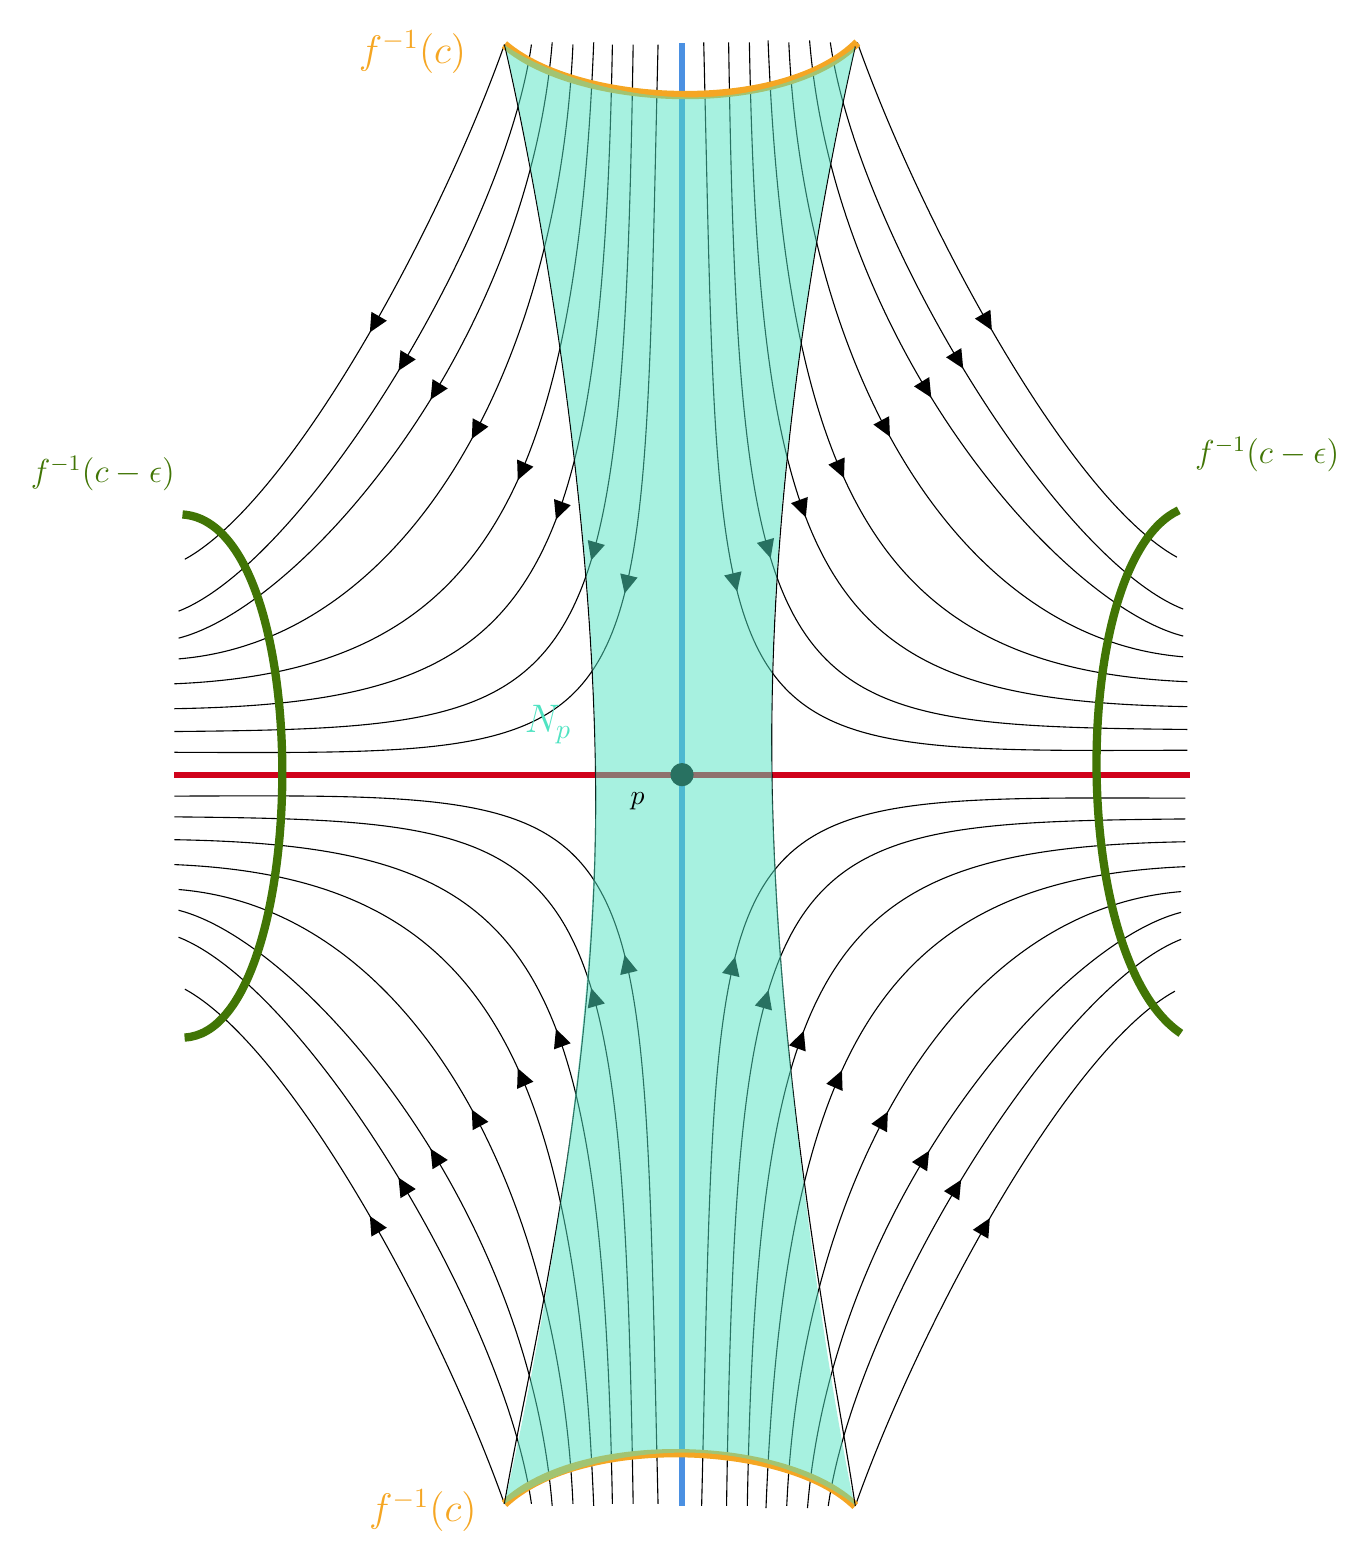
\begin{tikzpicture}[x=0.75pt,y=0.75pt,yscale=-1,xscale=1]
%uncomment if require: \path (0,843); %set diagram left start at 0, and has height of 843

%Straight Lines [id:da11875089429305197] 
\draw [color={rgb, 255:red, 74; green, 144; blue, 226 }  ,draw opacity=1 ][line width=2.25]    (329,31.6) -- (329,736.43) ;
%Straight Lines [id:da5325201497809933] 
\draw [color={rgb, 255:red, 208; green, 2; blue, 27 }  ,draw opacity=1 ][line width=2.25]    (84.42,384.02) -- (573.58,384.02) ;
%Shape: Circle [id:dp07579894054308489] 
\draw  [draw opacity=0][fill={rgb, 255:red, 0; green, 0; blue, 0 }  ,fill opacity=1 ] (323.4,384.02) .. controls (323.4,380.92) and (325.91,378.42) .. (329,378.42) .. controls (332.09,378.42) and (334.6,380.92) .. (334.6,384.02) .. controls (334.6,387.11) and (332.09,389.62) .. (329,389.62) .. controls (325.91,389.62) and (323.4,387.11) .. (323.4,384.02) -- cycle ;
%Curve Lines [id:da1665503577346341] 
\draw    (339.45,31.25) .. controls (347.8,378.2) and (336.45,373.05) .. (572.45,372.25) ;
\draw [shift={(355.57,295.75)}, rotate = 256.55] [fill={rgb, 255:red, 0; green, 0; blue, 0 }  ][line width=0.08]  [draw opacity=0] (8.93,-4.29) -- (0,0) -- (8.93,4.29) -- cycle    ;
%Curve Lines [id:da7994448259938868] 
\draw    (351.45,31.25) .. controls (356.45,355.25) and (373.45,360.25) .. (572.45,362.25) ;
\draw [shift={(371.68,279.76)}, rotate = 253.92] [fill={rgb, 255:red, 0; green, 0; blue, 0 }  ][line width=0.08]  [draw opacity=0] (8.93,-4.29) -- (0,0) -- (8.93,4.29) -- cycle    ;
%Curve Lines [id:da558792425961241] 
\draw    (361.45,31.25) .. controls (366.45,302.25) and (401.45,348.25) .. (572.45,351.25) ;
\draw [shift={(388.63,260.1)}, rotate = 249.87] [fill={rgb, 255:red, 0; green, 0; blue, 0 }  ][line width=0.08]  [draw opacity=0] (8.93,-4.29) -- (0,0) -- (8.93,4.29) -- cycle    ;
%Curve Lines [id:da5211576581151481] 
\draw    (370.45,30.25) .. controls (379.45,254.25) and (428.45,333.25) .. (572.45,339.25) ;
\draw [shift={(407.03,241.09)}, rotate = 246.23] [fill={rgb, 255:red, 0; green, 0; blue, 0 }  ][line width=0.08]  [draw opacity=0] (8.93,-4.29) -- (0,0) -- (8.93,4.29) -- cycle    ;
%Curve Lines [id:da39021575553782684] 
\draw    (380.45,31.25) .. controls (387.45,187.25) and (460.45,318.25) .. (570.45,327.25) ;
\draw [shift={(429.18,221.22)}, rotate = 242] [fill={rgb, 255:red, 0; green, 0; blue, 0 }  ][line width=0.08]  [draw opacity=0] (8.93,-4.29) -- (0,0) -- (8.93,4.29) -- cycle    ;
%Curve Lines [id:da6126506516051217] 
\draw    (390.45,30.25) .. controls (402.45,177.25) and (511.45,302.25) .. (570.45,317.25) ;
\draw [shift={(449.07,202.35)}, rotate = 238.74] [fill={rgb, 255:red, 0; green, 0; blue, 0 }  ][line width=0.08]  [draw opacity=0] (8.93,-4.29) -- (0,0) -- (8.93,4.29) -- cycle    ;
%Curve Lines [id:da24082042581971141] 
\draw    (400.45,31.25) .. controls (413.45,123.25) and (509.45,280.25) .. (570.45,304.25) ;
\draw [shift={(464.47,188.39)}, rotate = 239.04] [fill={rgb, 255:red, 0; green, 0; blue, 0 }  ][line width=0.08]  [draw opacity=0] (8.93,-4.29) -- (0,0) -- (8.93,4.29) -- cycle    ;
%Curve Lines [id:da5298362087143788] 
\draw    (413.45,31.25) .. controls (445.45,121.25) and (516.45,251.25) .. (567.45,279.25) ;
\draw [shift={(478.29,169.92)}, rotate = 240.15] [fill={rgb, 255:red, 0; green, 0; blue, 0 }  ][line width=0.08]  [draw opacity=0] (8.93,-4.29) -- (0,0) -- (8.93,4.29) -- cycle    ;

%Curve Lines [id:da21918221686589523] 
\draw    (317.45,32.25) .. controls (309.1,379.2) and (320.45,374.05) .. (84.45,373.25) ;
\draw [shift={(301.33,296.75)}, rotate = 283.45] [fill={rgb, 255:red, 0; green, 0; blue, 0 }  ][line width=0.08]  [draw opacity=0] (8.93,-4.29) -- (0,0) -- (8.93,4.29) -- cycle    ;
%Curve Lines [id:da34745008178206616] 
\draw    (305.45,32.25) .. controls (300.45,356.25) and (283.45,361.25) .. (84.45,363.25) ;
\draw [shift={(285.22,280.76)}, rotate = 286.08] [fill={rgb, 255:red, 0; green, 0; blue, 0 }  ][line width=0.08]  [draw opacity=0] (8.93,-4.29) -- (0,0) -- (8.93,4.29) -- cycle    ;
%Curve Lines [id:da8640093846313118] 
\draw    (295.45,32.25) .. controls (290.45,303.25) and (255.45,349.25) .. (84.45,352.25) ;
\draw [shift={(268.27,261.1)}, rotate = 290.13] [fill={rgb, 255:red, 0; green, 0; blue, 0 }  ][line width=0.08]  [draw opacity=0] (8.93,-4.29) -- (0,0) -- (8.93,4.29) -- cycle    ;
%Curve Lines [id:da925990106139973] 
\draw    (286.45,31.25) .. controls (277.45,255.25) and (228.45,334.25) .. (84.45,340.25) ;
\draw [shift={(249.87,242.09)}, rotate = 293.77] [fill={rgb, 255:red, 0; green, 0; blue, 0 }  ][line width=0.08]  [draw opacity=0] (8.93,-4.29) -- (0,0) -- (8.93,4.29) -- cycle    ;
%Curve Lines [id:da08743123557319321] 
\draw    (276.45,32.25) .. controls (269.45,188.25) and (196.45,319.25) .. (86.45,328.25) ;
\draw [shift={(227.72,222.22)}, rotate = 298] [fill={rgb, 255:red, 0; green, 0; blue, 0 }  ][line width=0.08]  [draw opacity=0] (8.93,-4.29) -- (0,0) -- (8.93,4.29) -- cycle    ;
%Curve Lines [id:da08430775562121551] 
\draw    (266.45,31.25) .. controls (254.45,178.25) and (145.45,303.25) .. (86.45,318.25) ;
\draw [shift={(207.83,203.35)}, rotate = 301.26] [fill={rgb, 255:red, 0; green, 0; blue, 0 }  ][line width=0.08]  [draw opacity=0] (8.93,-4.29) -- (0,0) -- (8.93,4.29) -- cycle    ;
%Curve Lines [id:da38820398572752524] 
\draw    (256.45,32.25) .. controls (243.45,124.25) and (147.45,281.25) .. (86.45,305.25) ;
\draw [shift={(192.43,189.39)}, rotate = 300.96] [fill={rgb, 255:red, 0; green, 0; blue, 0 }  ][line width=0.08]  [draw opacity=0] (8.93,-4.29) -- (0,0) -- (8.93,4.29) -- cycle    ;
%Curve Lines [id:da5677669307058717] 
\draw    (243.45,32.25) .. controls (211.45,122.25) and (140.45,252.25) .. (89.45,280.25) ;
\draw [shift={(178.61,170.92)}, rotate = 299.85] [fill={rgb, 255:red, 0; green, 0; blue, 0 }  ][line width=0.08]  [draw opacity=0] (8.93,-4.29) -- (0,0) -- (8.93,4.29) -- cycle    ;

%Curve Lines [id:da5375642083324416] 
\draw    (338.45,736.36) .. controls (346.8,389.41) and (335.45,394.56) .. (571.45,395.36) ;
\draw [shift={(354.57,471.87)}, rotate = 103.45] [fill={rgb, 255:red, 0; green, 0; blue, 0 }  ][line width=0.08]  [draw opacity=0] (8.93,-4.29) -- (0,0) -- (8.93,4.29) -- cycle    ;
%Curve Lines [id:da5126738644229648] 
\draw    (350.45,736.36) .. controls (355.45,412.36) and (372.45,407.36) .. (571.45,405.36) ;
\draw [shift={(370.68,487.86)}, rotate = 106.08] [fill={rgb, 255:red, 0; green, 0; blue, 0 }  ][line width=0.08]  [draw opacity=0] (8.93,-4.29) -- (0,0) -- (8.93,4.29) -- cycle    ;
%Curve Lines [id:da5839119584885231] 
\draw    (360.45,736.36) .. controls (365.45,465.36) and (400.45,419.36) .. (571.45,416.36) ;
\draw [shift={(387.63,507.52)}, rotate = 110.13] [fill={rgb, 255:red, 0; green, 0; blue, 0 }  ][line width=0.08]  [draw opacity=0] (8.93,-4.29) -- (0,0) -- (8.93,4.29) -- cycle    ;
%Curve Lines [id:da975815253328843] 
\draw    (369.45,737.36) .. controls (378.45,513.36) and (427.45,434.36) .. (571.45,428.36) ;
\draw [shift={(406.03,526.52)}, rotate = 113.77] [fill={rgb, 255:red, 0; green, 0; blue, 0 }  ][line width=0.08]  [draw opacity=0] (8.93,-4.29) -- (0,0) -- (8.93,4.29) -- cycle    ;
%Curve Lines [id:da9314613290760876] 
\draw    (379.45,736.36) .. controls (386.45,580.36) and (459.45,449.36) .. (569.45,440.36) ;
\draw [shift={(428.18,546.4)}, rotate = 118] [fill={rgb, 255:red, 0; green, 0; blue, 0 }  ][line width=0.08]  [draw opacity=0] (8.93,-4.29) -- (0,0) -- (8.93,4.29) -- cycle    ;
%Curve Lines [id:da09174306781681929] 
\draw    (389.45,737.36) .. controls (401.45,590.36) and (510.45,465.36) .. (569.45,450.36) ;
\draw [shift={(448.07,565.26)}, rotate = 121.26] [fill={rgb, 255:red, 0; green, 0; blue, 0 }  ][line width=0.08]  [draw opacity=0] (8.93,-4.29) -- (0,0) -- (8.93,4.29) -- cycle    ;
%Curve Lines [id:da21494064860512774] 
\draw    (399.45,736.36) .. controls (412.45,644.36) and (508.45,487.36) .. (569.45,463.36) ;
\draw [shift={(463.47,579.22)}, rotate = 120.96] [fill={rgb, 255:red, 0; green, 0; blue, 0 }  ][line width=0.08]  [draw opacity=0] (8.93,-4.29) -- (0,0) -- (8.93,4.29) -- cycle    ;
%Curve Lines [id:da5065198292397652] 
\draw    (412.45,736.36) .. controls (444.45,646.36) and (515.45,516.36) .. (566.45,488.36) ;
\draw [shift={(477.29,597.7)}, rotate = 119.85] [fill={rgb, 255:red, 0; green, 0; blue, 0 }  ][line width=0.08]  [draw opacity=0] (8.93,-4.29) -- (0,0) -- (8.93,4.29) -- cycle    ;

%Curve Lines [id:da3880154567702636] 
\draw    (317.45,735.36) .. controls (309.1,388.41) and (320.45,393.56) .. (84.45,394.36) ;
\draw [shift={(301.33,470.87)}, rotate = 76.55] [fill={rgb, 255:red, 0; green, 0; blue, 0 }  ][line width=0.08]  [draw opacity=0] (8.93,-4.29) -- (0,0) -- (8.93,4.29) -- cycle    ;
%Curve Lines [id:da9327211409936709] 
\draw    (305.45,735.36) .. controls (300.45,411.36) and (283.45,406.36) .. (84.45,404.36) ;
\draw [shift={(285.22,486.86)}, rotate = 73.92] [fill={rgb, 255:red, 0; green, 0; blue, 0 }  ][line width=0.08]  [draw opacity=0] (8.93,-4.29) -- (0,0) -- (8.93,4.29) -- cycle    ;
%Curve Lines [id:da09647590503157577] 
\draw    (295.45,735.36) .. controls (290.45,464.36) and (255.45,418.36) .. (84.45,415.36) ;
\draw [shift={(268.27,506.52)}, rotate = 69.87] [fill={rgb, 255:red, 0; green, 0; blue, 0 }  ][line width=0.08]  [draw opacity=0] (8.93,-4.29) -- (0,0) -- (8.93,4.29) -- cycle    ;
%Curve Lines [id:da15668737739736305] 
\draw    (286.45,736.36) .. controls (277.45,512.36) and (228.45,433.36) .. (84.45,427.36) ;
\draw [shift={(249.87,525.52)}, rotate = 66.23] [fill={rgb, 255:red, 0; green, 0; blue, 0 }  ][line width=0.08]  [draw opacity=0] (8.93,-4.29) -- (0,0) -- (8.93,4.29) -- cycle    ;
%Curve Lines [id:da5883237308999977] 
\draw    (276.45,735.36) .. controls (269.45,579.36) and (196.45,448.36) .. (86.45,439.36) ;
\draw [shift={(227.72,545.4)}, rotate = 62] [fill={rgb, 255:red, 0; green, 0; blue, 0 }  ][line width=0.08]  [draw opacity=0] (8.93,-4.29) -- (0,0) -- (8.93,4.29) -- cycle    ;
%Curve Lines [id:da9204033290837756] 
\draw    (266.45,736.36) .. controls (254.45,589.36) and (145.45,464.36) .. (86.45,449.36) ;
\draw [shift={(207.83,564.26)}, rotate = 58.74] [fill={rgb, 255:red, 0; green, 0; blue, 0 }  ][line width=0.08]  [draw opacity=0] (8.93,-4.29) -- (0,0) -- (8.93,4.29) -- cycle    ;
%Curve Lines [id:da49739155745577546] 
\draw    (256.45,735.36) .. controls (243.45,643.36) and (147.45,486.36) .. (86.45,462.36) ;
\draw [shift={(192.43,578.22)}, rotate = 59.04] [fill={rgb, 255:red, 0; green, 0; blue, 0 }  ][line width=0.08]  [draw opacity=0] (8.93,-4.29) -- (0,0) -- (8.93,4.29) -- cycle    ;
%Curve Lines [id:da32213499249738287] 
\draw    (243.45,735.36) .. controls (211.45,645.36) and (140.45,515.36) .. (89.45,487.36) ;
\draw [shift={(178.61,596.7)}, rotate = 60.15] [fill={rgb, 255:red, 0; green, 0; blue, 0 }  ][line width=0.08]  [draw opacity=0] (8.93,-4.29) -- (0,0) -- (8.93,4.29) -- cycle    ;


%Curve Lines [id:da05541171078629925] 
\draw [color={rgb, 255:red, 245; green, 166; blue, 35 }  ,draw opacity=1 ][line width=3]    (243.45,32.25) .. controls (279.42,63.08) and (378.33,66.67) .. (413.45,31.25) ;
%Curve Lines [id:da4989004892868002] 
\draw [color={rgb, 255:red, 245; green, 166; blue, 35 }  ,draw opacity=1 ][line width=3]    (243.45,735.36) .. controls (280.33,700.67) and (380.33,704.67) .. (412.45,736.36) ;
%Curve Lines [id:da44411839842500755] 
\draw [color={rgb, 255:red, 65; green, 117; blue, 5 }  ,draw opacity=1 ][line width=3]    (88.33,258.67) .. controls (154.22,262.97) and (150.33,507.67) .. (89.33,510.67) ;
%Curve Lines [id:da05367202270104565] 
\draw [color={rgb, 255:red, 65; green, 117; blue, 5 }  ,draw opacity=1 ][line width=3]    (568.33,256.67) .. controls (516.33,280.67) and (514.33,471.67) .. (569.33,508.67) ;
%Curve Lines [id:da7969530986481941] 
\draw    (243.45,32.25) .. controls (254.33,78.67) and (285.1,230.49) .. (287.33,382.67) .. controls (289.57,534.85) and (253.34,675.31) .. (243.45,735.36) ;
%Curve Lines [id:da5283140439270424] 
\draw    (412.45,33.25) .. controls (400.33,86.67) and (370.1,232.49) .. (372.33,384.67) .. controls (374.57,536.85) and (404.33,680.67) .. (412.45,736.36) ;

%Shape: Polygon Curved [id:ds3817941045439226] 
\draw  [draw opacity=0][fill={rgb, 255:red, 80; green, 227; blue, 194 }  ,fill opacity=0.5 ] (243.45,735.36) .. controls (243.39,735.01) and (288.33,547.67) .. (287.33,382.67) .. controls (286.33,217.67) and (244.39,31.96) .. (243.45,32.25) .. controls (242.51,32.54) and (278.33,56.67) .. (330.33,57.67) .. controls (382.33,58.67) and (412.39,33.99) .. (412.45,33.25) .. controls (412.51,32.51) and (368.33,212.67) .. (372.33,384.67) .. controls (376.33,556.67) and (411.01,736.21) .. (412.45,736.36) .. controls (413.89,736.52) and (381.33,709.67) .. (327.33,710.67) .. controls (273.33,711.67) and (243.51,735.72) .. (243.45,735.36) -- cycle ;

% Text Node
\draw (303,391.4) node [anchor=north west][inner sep=0.75pt]    {$p$};
% Text Node
\draw (172,24.4) node [anchor=north west][inner sep=0.75pt]  [font=\Large,color={rgb, 255:red, 245; green, 166; blue, 35 }  ,opacity=1 ]  {$f^{-1}( c)$};
% Text Node
\draw (177,727.07) node [anchor=north west][inner sep=0.75pt]  [font=\Large,color={rgb, 255:red, 245; green, 166; blue, 35 }  ,opacity=1 ]  {$f^{-1}( c)$};
% Text Node
\draw (14,229.4) node [anchor=north west][inner sep=0.75pt]  [font=\large,color={rgb, 255:red, 65; green, 117; blue, 5 }  ,opacity=1 ]  {$f^{-1}( c-\epsilon )$};
% Text Node
\draw (575,220.4) node [anchor=north west][inner sep=0.75pt]  [font=\large,color={rgb, 255:red, 65; green, 117; blue, 5 }  ,opacity=1 ]  {$f^{-1}( c-\epsilon )$};
% Text Node
\draw (252,349.4) node [anchor=north west][inner sep=0.75pt]  [font=\Large,color={rgb, 255:red, 80; green, 227; blue, 194 }  ,opacity=1 ]  {$N_{p}$};


\end{tikzpicture}


}
    \end{center}
Idea: Show it locally in a morse chart arround $p$. Hopefully we can archive, that in such a chart the property $\phi_T(x)\geq a-\epsilon$ translates to $x=\psi(x_s,x_u)$ where $\norm{x_u}\leq T_x$. Then assume $T$ to be big enough such that for any $x\in N_p$ there is a chart $U$ arround a point $x_p\in W(\to p)$ and a $t_0$ such that $\phi_{t_0}(U)$ lives in said morse chart. Finaly check if the property required arround said $x_p$ can be furmulated such that $U$ has a tubular structure.
So lets start this procedure! 
Let
\begin{align*}
    \psi:p\in V \to U \subseteq \R^m 
\end{align*} be a morse chart. Here the function $f$ is of the form
\begin{equation*}
    f\circ \psi^{-1} (x_s,x_u)=a+{x^s}^2-{x^u}^2\,. 
\end{equation*} where ${x^s}^2$ and ${x^u}^2$ denotes the sum of all the squares from the morse lemma. Without restrictions we call $x^s=(x^1,\dots x^l$ and $x^u:(x^{l+1},\dots x^m)$. Now we inspect the set 
\begin{equation} 
    \psi^{-1}(N_p\cap V)=\left\{(x^s,x^u)\in U~|~f\circ \phi_T(\psi^{-1}(x^s,x^ u))\geq a-\epsilon\right\} \, .
\end{equation} First we inspect the gradient in those local coordinats, i.e. $x=\psi^{-1}(u)$:
\begin{align*}
    \grad(f)(x)=g^{ik}~\frac{\partial f }{x^k}\frac{\partial}{x^i}
\end{align*} For now assume that $g_{ik}=\diag(1,\dots 1)$, i.e. that we work with the euklidean metric. Then the gradient is:
\begin{align*}
    \sum_{i,k} \frac{\partial f \circ \psi^{-1}}{\partial x^k} \frac{\partial}{\partial x^i}= 2\frac{\partial}{x^s} -2\frac{\partial}{x^u}\, .
\end{align*} Hence, the flow corresponding to $\psi_*(-\grad(f))$ is of the form
\begin{align*}
    t\mapsto \phi_t(x)=(e^{-2t}x^s,e^{2t}x^u) \, .
\end{align*} Assume that $\epsilon$ is small enough, such that all $x\in \psi(N_p\cap V)\setminus W(\to p)$ flow through $f^{-1}(a-\epsilon)$ inside of $U$, i.e. we can formulate the property:
\begin{equation}
    f\circ \phi_T(\psi^{-1}(x^s,x^ u))\geq a-\epsilon \quad \Leftrightarrow \quad f\left( \psi^{-1}(e^{-2T}x^s,e^{2T}x^u) \right)= a+{( e^{-2T}x^s)}^2-(e^{2T}x^u)^2  \geq a-\epsilon
\end{equation}
This however reads: 
\begin{align*}
     a+{( e^{-2T}x^s)}^2-(e^{2T}x^u)^2  \geq a-\epsilon  \quad \Leftrightarrow \quad (e^{2T}x^u)^2 \leq \epsilon+ {( e^{-2T}x^s)}^2 \, 
\end{align*}And hence we have that:
\begin{equation*}
    \psi(N_p\cap V)=\left\{(x^s,x^u)\in U ~\middle|~\norm{x^u}\leq R(x^s)\right\}
\end{equation*} where $R(x^s)$ is a smooth function. Now let $g$ be a general metric, and $\psi$ a Morse chart centered in $p$ such that $g(p)$ is a diagonal quadratic form with respect to that morse chart. We now want to interlinear approximate  $\psi\circ \phi_t \circ \psi^{-1}:U\to U$ which leads to the need of its jacobean. By lemma \ref{} together with the local form of the gradient we have the form:
\begin{align*}
	q_{\psi}	\frac{\partial}{\partial x}\big|_0 \phi_t(\psi^{-1}(x)	)
	&=\exp\left( \sum_k \left(g^{ki}(0) \frac{\partial ^2 (f\circ \psi^{-1})}{\partial x^j\partial x^k}\right)_{ij} \right) \, .
\end{align*} Now $g^{ki}(0)=\delta_{ik}\mu_k$ with $\mu_i>0$ for all $i$ and $\frac{\partial ^2 (f\circ \psi^{-1})}{\partial x^j\partial x^k}=s_{k} 2\delta_{jk}$ where $s_{k}=-1$ if $k\leq l$ and $s_k=1$ else. Hence: 
\begin{align*}
			\frac{\partial}{\partial x}\big|_0 \psi\circ \phi_t(\psi^{-1}(x)	)&=-\exp\left(\diag(-2\mu_1t,\dots,¸ -2\mu_lt,2\mu_{l+1}t,\dots,2\mu_mt)\right)\\ 
			&=\diag(\euler^{2\mu_{1}t},\dots \euler^{2\mu_{l}t},\euler^{-2\mu_{l+1}t},\dots,\euler^{-2\mu_{m}t}) 
\end{align*}
Hence we can linearly approximate the flow for fixed $t$ in a chart centered at the critical point to get a function $\mathcal{R}:V\to V$ such that $\mathcal{R}\in \mathcal{O}(\norm{x}^2)$:
\begin{align*}
	\psi\circ \phi_t(\psi^{-1})(x)
	&=\psi\circ \phi_t(\psi^{-1})(0)+\left( \frac{\partial}{\partial x}\big|_0	\psi\circ \phi_t(\psi^{-1})\right) x+\mathcal{R}(x)\\
	&=\left( \diag(\euler^{2\mu_{1}t},\dots \euler^{2\mu_{l}t},\euler^{-2\mu_{l+1}t},\dots,\euler^{-2\mu_{m}t}) \right)(x) +\mathcal{R}(x)
\end{align*}
We give the following definitions: 
\begin{itemize}
\item $x^u\coloneq (x^1,\dots,x^l)$ and $x^s \coloneq (x^{l+1},\dots x^m)$, and with this we split $x=(x^u,x^s)$.
\item $-(x^{u})^2\coloneq \sum _{i=1}^l-(x^l)^2$ and $(x^{s})^2\coloneq \sum_{i=l+1}^m (x^i)^2$ and hence 
\begin{align*}
	f\circ\psi^{-1}(x^u,x^s)=a-(x^{u})^2+(x^{s})^2\, .
\end{align*} 
\item  $\euler^{2\mu_u t}x^u\coloneq(\euler^{2\mu_{1}}x^1,\dots \euler^{2\mu_{l}}x^l)$ and similar $\euler^{-2\mu_s t }x^s\coloneq (\euler^{-2\mu_{l+1}}x^{l+1},\dots,\euler^{-2\mu_{m}}x^m)$.
\item $\mathcal{R}^u(x)$ and $\mathcal{R^s}(x)$ such that $\mathcal{R}(x)=\left(\mathcal{R}^u(x),\mathcal{R}^s(x)\right)$
\end{itemize} With these notations the calculation above yields:
\begin{align*}
\psi\circ \phi_t(\psi^{-1})(x)(x^u,x^s)=\left(\euler^{2\mu_ut}x^u+\mathcal{R}^u(x),\euler^{-2\mu_st}x^s+\mathcal{R}^s(x)\right)\, .
\end{align*}
Now the property of being in $\psi(N_p\cap U)$ reads:
\begin{align*}
	\begin{array}{lll}
		x\in V \text{ such that } & f(\phi_T (\psi^{-1}(x))) & \leq a-\epsilon \\
		&\Leftrightarrow (f\circ \psi^{-1})(\psi\circ \phi_T (\psi{-1}(x)))& \leq a-\epsilon \\
		&\Leftrightarrow  (f\circ \psi^{-1})\left(\euler^{2\mu_uT}x^u+\mathcal{R}^u(x),\euler^{-2\mu_sT}x^s+\mathcal{R}^s(x)\right)&\leq a-\epsilon \\
		&\Leftrightarrow -\left(-\euler^{2\mu_uT}x^u+\mathcal{R}^u(x)\right)^2    
		+\left(\euler^{-2\mu_sT}x^s+\mathcal{R}^s(x)\right)^2+\epsilon &\leq 0
	\end{array}
\end{align*} 
We now inspect the funktion $F:\R^m\to \R^l$ given by:
\begin{equation*}
\left(\begin{array}{l}
	x^1\\ \vdots \\x^m
\end{array}\right) \mapsto	\left(\begin{array}{cccc}
		-\left(\euler^{2\mu_{1}T}x^{1}\right)^2&+2\euler^{2\mu_{1}T}x^{1}\mathcal{R}^1(x)&+\left(\mathcal{R}^{1}(x)\right)^2&	+\left(\euler^{-2\mu_sT}x^s+\mathcal{R}^s(x)\right)^2\\
		\vdots &\vdots&\vdots&\\ 
		-\left(\euler^{2\mu_{l}T}x^{l}\right)^2&+2\euler^{2\mu_{l}T}x^{l}\mathcal{R}^l(x)&+\left(\mathcal{R}^{l}(x)\right)^2&\\
	\end{array}\right)\, .
\end{equation*} For this funktion we have that 
\begin{align*}
\frac{\partial}{\partial x^s}F
\end{align*} is non-degenerat. For this we need to calculate the jacobean 
\end{proof}


\begin{comment}[Müll]
	\begin{lemma}
		If $(x_1,...,x_m)$ is a local coordinate system arround a critical point $p\in M$ and let $\left( \frac{\partial}{\partial x_1},\dots ,\frac{\partial}{\partial x_m}\right)$ be the induced basis of $T_pM$.  Then the Matrix of the differential of the gradient $\grad(f): U \to \R^m$ inj $p$ is of the form:
		\begin{align*}
			\frac{\partial}{\partial x}\grad(f)\Big|_p=\left(\sum_{k} g^{ki}\frac{\partial ^2 f }{\partial x_j \partial x_k} \right)_{ij}
		\end{align*}
	\end{lemma}
	
	\begin{proof}
		Compare lemma 4.4 in \cite{banyaga2004lectures}: 
		First we notice, that in the coordinates $x_1,...,x_n$ respectifly $(\frac{\partial}{\partial x_1},\dots \frac{\partial}{\partial x_m})$(given by the chart $\psi: U\to V$ )the $\grad(f)\circ \psi^{-1}$ reads:
		\begin{align*}
			Q\circ \grad(f)\circ \psi^{-1}= \left(\sum_k g^{k1}\frac{\partial f \circ \psi}{\partial x_k},\sum_k g^{k2}\frac{\partial f \circ \psi}{\partial x_k},\dots, \sum_k g^{km}\frac{\partial f \circ \psi}{\partial x_k} \right)
		\end{align*} Where $Q:TU\to \R^m$ denotes the koordinate map with respect to the chart on $\psi$. 
		Hence, we can differentiate: 
		\begin{align*}
			\frac{\partial}{\partial x}  Q\circ \grad(f)\circ \psi^{-1}
			&= \left(\frac{\partial}{\partial x_j} \sum_k g^{ki}\frac{\partial f \circ \psi}{\partial x_k}\right)_{ij} \\
			&= \left(\sum_k \left[ 
			\frac{\partial g^{ki}}{\partial x_j}\frac{\partial f \circ \psi}{\partial x_k} +  g^{ki}\frac{\partial^2 f \circ \psi}{\partial x_j ~\partial x_k}
			\right]\right)_{ij} \, .
		\end{align*} Hence, in a critical point $p=\psi^{-1}(x_0)$ we have that:
		\begin{align*}
			\frac{\partial}{\partial x}  Q\circ \grad(f)\circ \psi^{-1} \Big|_{x_0}=\left(\sum_k \left[ 
			g^{ki}(0)\frac{\partial^2 f \circ \psi}{\partial x_j ~\partial x_k}
			\right]\right)_{ij} \, .
		\end{align*} The last line is the precice notion of the lemma.
	\end{proof}
	.
	
	
	Now assume that $(x_1,...,x_m)$ is a morse chart, hence $f(x_1,...,x_m)=\sum_{i=1}^lx_i^2-\sum_{i=l+1}^mx_i^2$ and thereby in this chart:
	\begin{align}
		\frac{\partial ^2 f }{\partial x_j \partial x_k}= \begin{cases}
			\phantom{-} \delta_{ik}2& \text{ if } i\leq l \, , \\
			-\delta_{ik}2& \text{ else} \, .
		\end{cases}
	\end{align} This lets us calculate: 
	\begin{align*}
		\frac{\partial}{\partial x}\grad(f)\Big|_p=\begin{pmatrix}
			2 g^{11}  &  2g^{12}&   \dots   &  2g^{1m}\\
			\vdots    & \vdots  & \vdots    & \vdots \\
			2 g^{l1}  &  2g^{l2}&   \dots   &  2g^{lm}\\
			- 2 g^{l+11} &  -2g^{l+12}&   \dots   &  -2g^{l+1m}\\
			\vdots    & \vdots  & \vdots    & \vdots \\
			- 2 g^{m1} &  -2g^{m2}&   \dots   &  -2g^{mm}\\
		\end{pmatrix}
	\end{align*}
	
	
	
	
	
	
	\begin{corollary}
		Let $p$ be a critical point of a Morse function $f$ on a manifold $M$ and let $g(p)$ be the Riemannian metric on $T_pM$. Then there exists a Morse chart $\psi$ arround $p$ such that the representation of $g(p)$ in the basis induced by the Morse chart is given by a a diagonal matrix $diag(\mu_1,\dots \mu_m)$ with $\mu_i>0$ for all $i$ .
	\end{corollary}
	\begin{proof}
		The quadratic form of $f \circ \psi^{-1} - f(p)$ in the coordinates of the Morse chart is $q_H(v) = v^T H v$. The quadratic form induced by the Riemannian metric $g(p)$ is $q_G(v) = v^T G v$, where $v \in \mathbb{R}^m$ are the coordinate vectors. Since $g(p)$ is positive definite, $G$ is also positive definite, and $H$ is symmetric.
		
		Consider the generalized eigenvalue problem $Hv = \lambda G v$. Since $H$ and $G$ are real symmetric matrices and $G$ is positive definite, this problem has $m$ real eigenvalues $\lambda_1, \dots, \lambda_m$ and corresponding eigenvectors $v_1, \dots, v_m$, which can be chosen to be orthogonal with respect to the bilinear form defined by $G$, such that $v_i^T G v_j = \delta_{ij}$, since if $v_i$ and $v_j$ are different eigenvectors with respect to different eigenvalues, we can calculate:
		\begin{align*}
			v_j^THv_i=(Hv_j)^Tv_i=\lambda _j(Gv_j)^Tv_i=\lambda _j v_j^T G(v_i)  \quad \text{and}\quad 	v_j^THv_i= v_j^T \lambda_i G(v_i)=\lambda_i v_j^TG(v_i) \, .
		\end{align*} Hence we have the equality
		\begin{align*}
			\lambda _j(Gv_j)^Tv_i=\lambda_i v_j^TG(v_i) \Leftrightarrow \underbrace{(\lambda_j-\lambda_i)}_{\neq 0}v_j^T G(v_i)=0
		\end{align*} Hence all eigenspaces are orthogonal and we can use Gram Schmitt to make the bases of the eigenspaces orthogonal and by rescaling orthonormal.
		
		Let $L = [v_1 | \dots | v_m]$ be the matrix whose columns are these $G$-orthnormal eigenvectors. The linear change of coordinates	$y = Lz$ leads to new coordinates $z$. In these new coordinates, the quadratic forms transform as follows:
		\begin{align*}
			q_G(y) &= y^T G y = (Lz)^T G (Lz) = z^T L^T G L z = z^T I z = \sum_{i=1}^m z_i^2 \\
			q_H(y) &= y^T H y = (Lz)^T H (Lz) = z^T L^T H L z
		\end{align*}
		Since $H v_i = \lambda_i G v_i$, we have $L^T H L = \text{diag}(\lambda_1, \dots, \lambda_m)$. The eigenvalues $\lambda_i$ are real and have the same signature as the eigenvalues of $H$ ($l$ negative, $m-l$ positive), which is due to Sylvesters law of innertia.  By a further scaling of the coordinates $z$, the matrix $L^T H L$ can be brought into the form $\text{diag}(-1, \dots, -1, 1, \dots, 1)$. (by doing this however, the matrix $G$ becomes $G=\diag(\mu_1,\dots \mu_m)$ with $\mu_j>0~\forall j$) Hence, we have a morse chart.
	\end{proof}
	
	Now we want to calculate $\frac{\partial}{\partial x} \phi_t \Big| _p$ in such a Morse chart:
	For this we start by differentiating in $t-direction$:
	\begin{align*}
		\frac{\diff}{\diff t}\phi_t(x)=-\grad(f)(\phi_t(x))
	\end{align*} If we first differentiate this in $x-$direction and then in $t$ dircetion we have:
	\begin{align*}
		\frac{\diff }{\diff t} \frac{\partial}{\partial x}\phi_t(x)
		& =  \frac{\partial }{\partial x} \left( \frac{\partial}{\partial t}\phi_t(x) \right)\\
		& =  \frac{\partial }{\partial x} \left( -\grad(f)(\phi_t(x)) \right)         \\
		& = -\frac{\partial }{\partial x} \grad(f)(\frac{\partial }{\partial x}\phi_t(x)) \, .
	\end{align*}    In other words: $\Psi(t,x)\coloneq \frac{\partial}{\partial x}\phi_t(x)$ is a solution of the system of linear ordinary differential equations
	\begin{align*}
		\frac{\diff}{\diff t}\Psi(t,x)=-\frac{\partial }{\partial x} \grad(f)(\Psi(t,x)) \, , \\
		\Psi(0,x)= 1_{m\times m} \, .
	\end{align*} By the uniqueness of such systems we have that 
	\begin{align*}
		\Psi(t,x)=\exp\left(-\frac{\partial}{\partial x}\grad(f)\cdot t\right) \,.
	\end{align*} Now choose an orthonormal basis $B=(b_1,\dots b_m)$ of $T_pM$ with resprect to the bilinear form $g(p)(\psi^{-1}\oplus \psi^{-1}=:\R^m\oplus \R^m \to \R$. Since for a chart that is centered in $p$ the family 
	\begin{align*}
		\left(\frac{\partial}{\partial x^i}\right)_i
	\end{align*} forms a basis, there is a unique base change between the two bases, that can be realized as a linear change of coordinates in the following way:
	Define $\lambda^i_k\in \R$ such that $b_i=\sum_k\lambda^k_i (\frac{\partial}{\partial x^k})$. With this we define the linear map $L:\R^m\to \R^m$ by $x\mapsto \left((\lambda ^i_k)_{ik}\right)^{-1}x$. If we define $(L^{-1})_i$ to be the ith component of the inverse map, we have
	\begin{align*}
		\frac{\partial (L^{-1})_i}{\partial x^j}= \frac{\partial (\sum_k \lambda^i_k\cdot x^k)}{\partial x^j}= \lambda^i_j \, .
	\end{align*}Hence, the basis 
	$$\left(\frac{\partial}{\partial \tilde{x} ^i}\right)_i$$
	corresponding to the new chart $\psi\circ L: U\to V\subseteq \R^m$ reads for any $f_p\in \mathcal{E}_p(M)$:
	\begin{align*}
		\frac{\partial}{\partial \tilde{x} ^j}(f_p)
		& =\frac{\partial}{\partial x^j} \Big|_{0}(f\circ\psi^{-1}\circ L^{-1}) \\
		&= \sum _k \frac{\partial f\circ \psi^{-1}}{\partial x^k}(L^{-1}(0))\frac{\partial (L^{-1})_k}{\partial x^j}(0)\\
		&= \sum _k \underbrace{\frac{\partial f\circ \psi^{-1}}{\partial x^k}(0)}_{=\frac{\partial}{\partial x^k}(f_p)}  \underbrace{\frac{\partial (L^{-1})_k}{\partial x^j}(0)}_{=\lambda^k_j}\\
		& =\left(\sum_k \lambda^k_j(\frac{\partial}{\partial x^k})\right)(f_p)=b_j(f_p) \, .
	\end{align*} Hence, a linear change of koordinates lets us manipulate any chart such that the basis of the tangendspaces in the origin of the given chart is orthongonal (or even orthonormal) with resprect to a given metric.
	
	
	Now this is somewhat troublesome:
	We could now choose a basis, such that $\frac{\partial}{\partial x}\grad(f)$ is diagonal and hence the exponential is easy to calculate. But then we dont know how $f$ looks like. But with a Morse chart (where we controle $f$) we have trouble calculating the exponential of $\frac{\partial}{\partial x}\grad(f)$. The hope ist that there is a change of basis that keeps the splitting.
	
	
	
	We calculate $ g(p)\left( \frac{\partial}{\partial x_i}\big|_p, \frac{\partial}{\partial x_j}\big|_p\right)$. With the coordinate map we have that $g(p)\left(q_{\psi\circ L^{-1}}^{-1},q_{\psi\circ L^{-1}}^{-1}\right)$ is a quadratic form on $R^n$ and given by a matrix $\tilde{G}$. \todo{Check how $\tilde{G}$ and $G$ are connected, by analysing how $q_{\psi\circ L^{-1}}$ and $q_{\psi}$ are connected}
	
	
\end{comment}
